

\section{Sous-fonctions d'allocation}
\label{repl:sec:suballocation}

Une fonction d'allocation optimale nécessite la connaissance du nombre et de la
position des éditions successives. La fonction peut alors allouer des
identifiants dont la taille est logarithmique comparé à celle du
document. Malheureusement, aucune de ces deux informations n'est disponible dans
l'édition collaborative en temps réel. Dans ces conditions, nous supposerons que
le comportement d'édition est une suite d'éditions adjacentes les unes des
autres -- comme l'édition en tête ou l'édition en fin -- ou à des positions
aléatoires, ou enfin, une composition de ceux-ci.

Afin de gérer ces types d'édition, employer une fonction d'allocation conçue
pour l'édition en fin ne suffit pas. \TODO{Moar. Maybe merge the choice.}

\begin{figure}
  \centering
  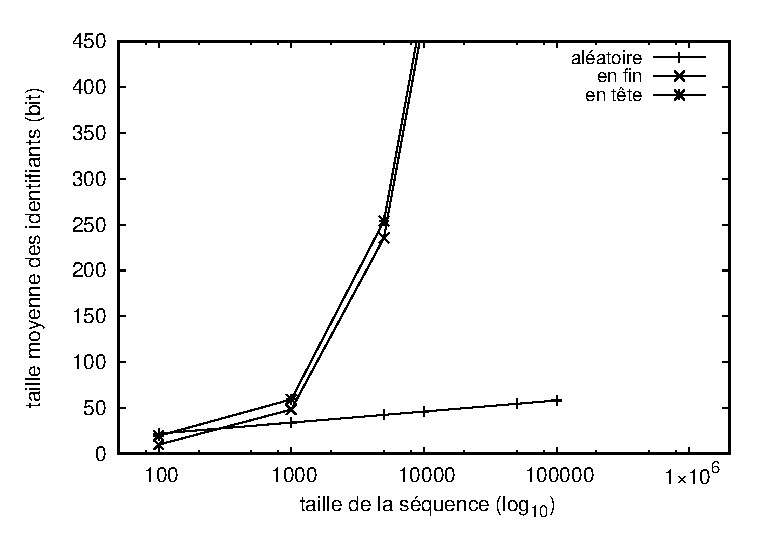
\includegraphics[width=0.8\textwidth]{img/lseq/robin.eps}
  \caption{\label{repl:img:suballocation} Arbre à arité constante et deux
    sous-stratégies d'allocation. L'axe des abscisses montre la taille du
    document sur une échelle logarithmique en base décimale. L'axe des ordonnées
    montre la moyenne des tailles des chemins alloués.}
\end{figure}

\begin{itemize}
\item [\textbf{Objectif :}] Montrer que deux sous-fonctions d'allocation conçues
  avec des objectifs antagonistes mais utilisées ensemble gèrent les
  comportements d'édition triviaux. Montrer que la progression des identifiants
  reste linéaire comparé à la taille du document.
\item [\textbf{Description :}] La simulation concerne trois documents
  grossissant au rythme des opérations d'insertions effectuées respectivement en
  tête, en fin, et aléatoirement. L'arbre a une arité maximale constante. Chaque
  niveau se voit attribuer une sous-fonction d'allocation, i.e., les niveaux
  pairs avec une fonction adaptée à l'édition en tête, et les niveaux impairs
  avec une fonction adaptée à l'édition en fin. Nous mesurons la moyenne des
  chemins composant les identifiants à 100, 1k, 5k, 10k, 50k, 100k insertions.
\item [\textbf{Résultat :}] La figure~\ref{repl:img:suballocation} montre les
  résultats obtenus à la suite de ces simulations. Nous observons tout d'abord
  que les chemins reste logarithmique sous un comportement d'édition
  aléatoire. Nous observons aussi que pour l'édition en tête et l'édition en
  fin, la progression est linéaire mais surtout, quasiment identique dans les
  deux cas.
\item [\textbf{Explication :}] Tout comme pour la
  figure~\ref{repl:img:exponentialtree}, l'édition à des positions aléatoire à
  pour effet d'équilibrer l'arbre représentant le document répliqué. Les chemins
  résultant de ce comportement grandissent de manière logarithmique. Grâce à une
  alternance des sous-fonctions d'allocation, la taille des chemins alloués lors
  de l'édition en tête ou en fin augmente lentement. Malgré tout, la progression
  reste linéaire. De plus, elle augmente deux fois plus rapidement que sans
  cette alternance avec un comportement d'édition favorable. En effet, dans le
  cas de ces simulations, un niveau sur deux composant un chemin est perdu car
  consommé trop vite : la sous-fonction d'allocation assignée à ce niveau
  n'était pas celle conçue pour le comportement d'édition courant.
\end{itemize}

